%% LaTeX template for BSc Computing for Games final year project dissertations
%% by Edward Powley
%% Games Academy, Falmouth University, UK

%% Based on:
%% bare_jrnl.tex
%% V1.4b
%% 2015/08/26
%% by Michael Shell
%% see http://www.michaelshell.org/
%% for current contact information.
%%
%% This is a skeleton file demonstrating the use of IEEEtran.cls
%% (requires IEEEtran.cls version 1.8b or later) with an IEEE
%% journal paper.
%%
%% Support sites:
%% http://www.michaelshell.org/tex/ieeetran/
%% http://www.ctan.org/pkg/ieeetran
%% and
%% http://www.ieee.org/

%%*************************************************************************
%% Legal Notice:
%% This code is offered as-is without any warranty either expressed or
%% implied; without even the implied warranty of MERCHANTABILITY or
%% FITNESS FOR A PARTICULAR PURPOSE! 
%% User assumes all risk.
%% In no event shall the IEEE or any contributor to this code be liable for
%% any damages or losses, including, but not limited to, incidental,
%% consequential, or any other damages, resulting from the use or misuse
%% of any information contained here.
%%
%% All comments are the opinions of their respective authors and are not
%% necessarily endorsed by the IEEE.
%%
%% This work is distributed under the LaTeX Project Public License (LPPL)
%% ( http://www.latex-project.org/ ) version 1.3, and may be freely used,
%% distributed and modified. A copy of the LPPL, version 1.3, is included
%% in the base LaTeX documentation of all distributions of LaTeX released
%% 2003/12/01 or later.
%% Retain all contribution notices and credits.
%% ** Modified files should be clearly indicated as such, including  **
%% ** renaming them and changing author support contact information. **
%%*************************************************************************


\documentclass[journal]{IEEEtran}

\usepackage{graphicx}
% Insert additional usepackage commands here
\graphicspath{ {Figures/} }

\begin{document}
%
% paper title
% Titles are generally capitalized except for words such as a, an, and, as,
% at, but, by, for, in, nor, of, on, or, the, to and up, which are usually
% not capitalized unless they are the first or last word of the title.
% Linebreaks \\ can be used within to get better formatting as desired.
% Do not put math or special symbols in the title.
\title{ How Does Visualising Path-finding in an NPC Effect How Participants Explore a Level?}
%
%
% author name
\author{1507866}

% The paper headers -- please do not change these, but uncomment one of them as appropriate
% Uncomment this one for COMP320
\markboth{COMP320: Research Review and Proposal}{COMP320: Research Review and Proposal}
% Uncomment this one for COMP360
% \markboth{COMP360: Dissertation}{COMP360: Dissertation}

% make the title area
\maketitle

% As a general rule, do not put math, special symbols or citations
% in the abstract or keywords.
\begin{abstract}
The abstract goes here.
\end{abstract}

\section{Introduction}
% The very first letter is a 2 line initial drop letter followed
% by the rest of the first word in caps.
% 
% form to use if the first word consists of a single letter:
% \IEEEPARstart{A}{demo} file is ....
% 
% form to use if you need the single drop letter followed by
% normal text (unknown if ever used by the IEEE):
% \IEEEPARstart{A}{}demo file is ....
% 
% Some journals put the first two words in caps:
% \IEEEPARstart{T}{his demo} file is ....
% 
% Here we have the typical use of a "T" for an initial drop letter
% and "HIS" in caps to complete the first word.
\IEEEPARstart{T}{he} research questions proposed in this project are: how does visualising \textit{Rapidly Exploring Random Trees} (RRT) path finding in a \textit{Non Player Character} (NPC) affect how a player explores a game level?

This project will look at visualising an enemy NPC's path-finding using RRT based path-finding. Figure \ref{KuffnerRRT} shows an example of RRT path-finding where the RRT explores the area and then a path is drawn along the tree \cite{Kuffner2000}.  The visualisation will occur around an enemy NPC allowing the participant to see where the enemy is going. Logging tools in the play testing software will record how long a player spends in a level and what percent of the level they explore. This data will be used to see if the visualisation has any effect on how the participant explores the level of the given game. 

Previous papers have researched visualising \textit{Artifical Intelligence} (AI) and foregrounding AI. However, there is little on on what effect this has on how the participants play the game.


\subsection{Hypothesis:}
\textbf{Null Hypothesis}: Visualising RRT path-finding has no effect on the percent of the level the participant explores. \\
\textbf{Hypothesis 1}: Visualising RRT significantly effects the percent of the level the participant explores. \\
\textbf{Hypothesis 2}: Decreasing the size of rooms decreases the percent of the level explored. \\ 
\textbf{Hypothesis 3}: Varying size of RRT visualisation effects? 
Percent of level explored and/or time spent in level??


\section{Related Work}
\subsection{Foregrounding and Visualising AI}
% Foreground visualising AI
AI is used in most modern digital games. However, it is rarely foregrounded or visualized in those games.  Treanor~\textit{et al} say that the AI in games if often designed to fit the game. Therefore, this AI is supporting the game play rather than being central to it~\cite{treanor2015, eladhari2011}.  \\

Treanor~\textit{et al} surveyed many games that foreground AI in different ways.  From this they proposed a series of design patterns for foregrounding AI in digital games. 
The two design patterns relevant to this project are firstly ``AI as a Villain".  They describe this pattern as having the AI not try to outright defeat the player. Instead it's designed to create an experience like Alien Isolation~\cite{game:AlienIsolation, treanor2015}.  In Alien Isolation the AI hunts the player. This foregrounded appears here as the player has to observe the AI and learn how to avoid. 

This paper will also use AI as a villain as enemy NPC's  will have their path-finding visualized around them. The participants will have to observe this to learn how to not get caught by the enemy NPC.  


The second relevant design pattern is ``AI is Visualized". This is where there is a visual representation of the AI's state or decision making in the game. 

Most games hide this from the player but this design pattern visualizes it making it mechanic.  
The example given by Treanor \textit{et al} is the game Third Eye Crime.  Third Eye Crime is a game that followed the ``AI is Visualised" design pattern~\cite{Isla2014, game:ThirdEyeCrime}.  
The game uses probabilistic object tracking through Occupancy maps. The game uses Occupancy Maps to display where the enemy thinks the player could be in the map, as the enemy moves around the map it removes areas where the player is not from the Occupancy Map~\cite{Isla2014}.  Generally stealth games involve avoiding enemies,  this design encourages the player to trigger the mechanic allowing them to use the visualisation to mislead and avoid the enemy \cite{Isla2014, game:ThirdEyeCrime}.  

This pattern is relevant to this project as the enemy NPC will have RRT path-finding visualized around it. Allowing the player to see where the enemy is going and decide how to overcome or outsmart it.

% Tidied up to here
% Visualising in general
While Haworth \textit{et al} do not visualise an AI process they do visualise the possible decision in a game on a tree structure~\cite{Haworth2010}. They research visualising decision trees in a game to see what effect it had on children's analytical reasoning and game play.  While they did not come to any definite conclusions their results suggested that data aided players in playing the game as in later level the children struggled to beat the game without the visualised tree. However, an issue they noted was that the game could be unbalanced at the end making the usefulness of the tree being questionable.  

A further issue is that Haworth~\textit{et al} only tested the tree in a relatively simple 2D game that was tested on children. This does not give any data on 3D games on the market??? In contrast, Isla's visualised path-finding in Third Eye Crime is on sale?? (Word it better)~\cite{Isla2014}.
 
Like  Haworth \textit{et al}, Bauer \textit{et al} also research visualising tree structures~\cite{bauer2012}. However, they did use an AI technique, they used Rapidly-Exploring Random Trees (RRT).

\subsection{Pathfinding}
% A* / pathfinding in games
%  Expand this section
In digital games the A* path finding algorithm appears to be the most widely used~\cite{Algfoor2015}.  Algfoor \textit{et al} surveyed numerous papers on path finding. The focus appeared to be on the type of grids used in path-finding and then numerous algorithms that can be used~\cite{Algfoor2015}. The most popular being the A* algorithm for use in digital games and robotics. RRT path-finding was not mentioned. 
They surveyed many grid types and gave the advantages of each. However, RRT does not use grids it instead uses nodes making the grid type irrelevant.\\

Hu~\textit{et al} propose an implementation of A* path-finding in Unity, the engine being used by this project~\cite{Hu2012}.  While their implementation is in an older version Unity the implementation in Unity 5.6 should still be similar. 

Third Eye Crime was previously mentioned for it's foregrounding of AI. However, it also uses visualisation as an important mechanic~\cite{Isla2014}~\cite{ game:ThirdEyeCrime}. Isla uses Occupancy Maps to show where the enemy NPC thinks the player could be. Occupancy or Influence maps do not produce a path instead they show the probability of the player being in different locations across the map~\cite{Isla2014, Miles2006}. Isla used Occupancy maps to show where the enemy AI thinks the player currently is. He then used ....... for the NPC to navigate to the most likely location of the player. Similarily, Miles and Loius used also used influence maps. While their example is specific to \textit{Real Time Stratedgy} (RTS) games like Isla they used Occupancy maps as a base to for A* path-finding instead of A* using the map itself for path-finding~\cite{Miles2006}.\\
 
A further paper on path finding is Wang and Lu's paper which looks at path finding in a 3D environment. While again they were using A* they look at using A* in 3D and suggest using nodes instead of a grid??~\cite{wang2012}.

Mendonça~\textit{et al} look at path-finding both in robotics and digital games~\cite{Mendonça2015}. Their focus is on stealth path-finding in games and applying that to robotics. Like RRT, the methods they propose does not necessarily find the optimal path~\cite{karaman2010}~\cite{Mendonça2015}. They tried to find the most stealthy path. They generated custom navigation meshes (navmeshes) and assigned a weight to each polygon in the navmesh depending on how close it is to cover. 

As Mendonça~\textit{et al} as use path-finding to find a stealthy path the path with the optimal distance may not always be the path with the lowest cost in relation to the robot or AI agent staying cover. Therefore, the optimal path may not always be required. 

This project will favour interesting visualisations over the optimal path in the variant that uses   

^^ point is optimal not always necessary ^^
\\

navmeshes \cite{Hale2008} \cite{Mendonça2015}
%  RRT
%  Expand this section
Rapidly-Exploring Random Trees~(RRT) are a search method used more widely in robotics than digital games~\cite{LaValle1998}~\cite{Kuffner2000}. Kuffner and LaValle first proposed RRT in 2000, they intended to produce a random algorithm more efficient than the other search algorithms available at the time. Figure~\ref{KuffnerRRT} shows  Kuffner and LaValle's RRT Path Planner a variant of RRT that can be used to find paths from the generated tree~\cite{Kuffner2000}.

\begin{figure}[h]
	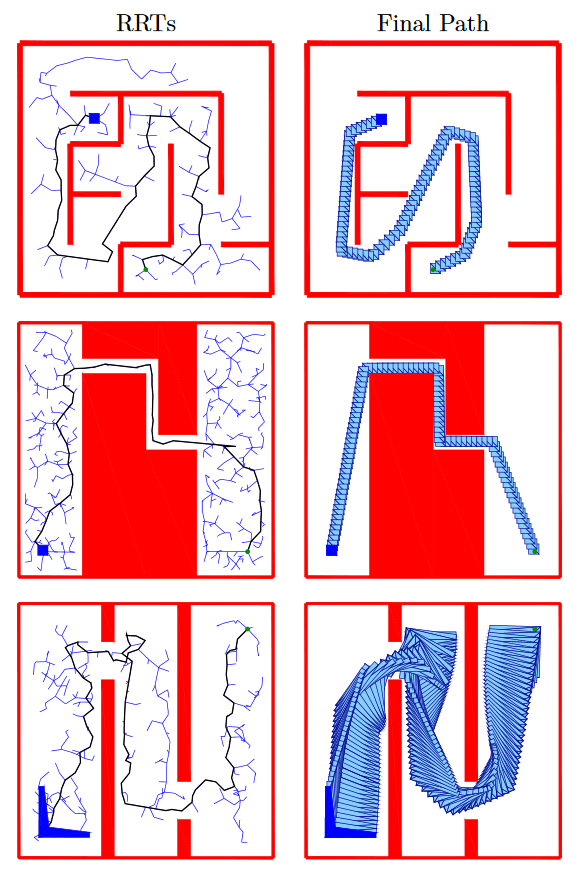
\includegraphics[width=1.0\linewidth]{KuffnerRRT.png}
	\caption{ Kuffner and LaValle's \cite{Kuffner2000}.}
	\label{KuffnerRRT}
\end{figure} 


RRT's goal is to find a path between two point with no collisions, the path found may not the the optimal path though~\cite{Kuffner2000, Karaman2011}.  Karaman and Sertac say that the chance of RRT finding an optimal path is very unlikely~\cite{karaman2010}.  Karaman \textit{et al} propose another version of RRT called RRT* this version 

%  RRT & games
Bauer and Popovic used RRT for level design in games~\cite{bauer2012}. Like Haworth \textit{et al} they visualised the data to aid users~\cite{bauer2012}~\cite{Haworth2010}. However unlike Haworth \textit{et al} the visualisation is for game developers not the players. 

\begin{figure}[h]
	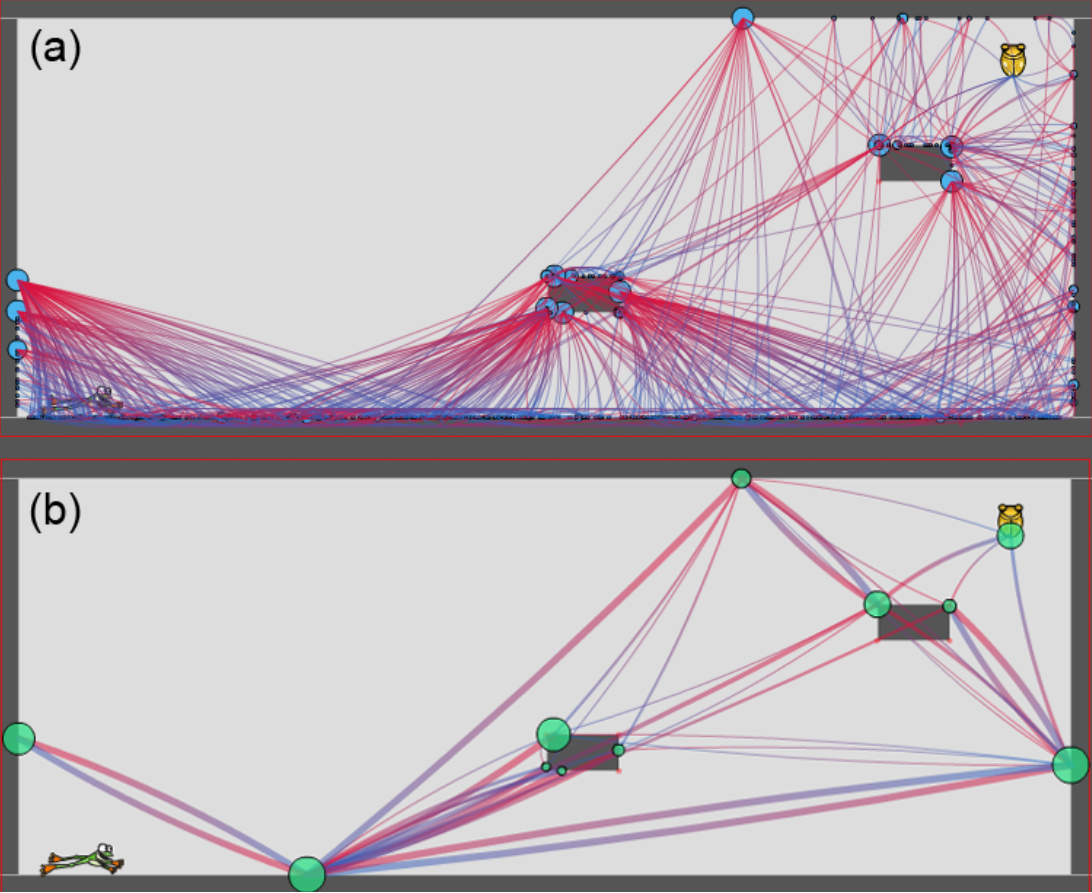
\includegraphics[width=1.0\linewidth]{BauerRRT.png}
	\caption{ Bauer \textit{et al}'s graph-based representation of RRT with and without clustering \cite{bauer2012}.}
	\label{BauerRRT}
\end{figure} 

Their focus is on level design not game-play. They designed a tool that could analyse a level generated by PCG or a level designer. They then use RRT to calculate possible routes the player could take when playing. This produced an image that was difficult to read so Dongen's method is used for graph clustering to make the output more legible~\cite{bauer2012, van2001}.  This project is focused on using the visualisation in the game to the game design. However, a similar technique will be required to organise the RRT output to make it understandable to the player in way that they can look at the visualisation and interpret what the NPC is going to do. 


% RRT vs  A*
A* and optimal paths vs RRT better visualisation 


\subsection{Exploring Game Environments}
% Wayfinding
One method of guiding players through games is to use wayfinding. Wayfinding in games is often visual cues in the environment that will guide the player to an area of interest~\cite{si2017, Bacim2008}. While the intention of visualising the RRT path-finding is not to guide players through a level but one of the behaviours being observed in participants is whether they  navigate or explore differently with the presence of visible path-finding. 

Moura and Bartram investigated the effects different wayfinding cues have on players~\cite{moura2014}.  They looked at methods used in AAA games and mimicked them in their own game. Their results showed that the absence of wayfinding cues was obvious to players. In contrast the version with wayfinding cues did not have enough cues to sufficiently guide the player. These results suggest that wayfinding cues alone may not be enough to guide the player. While the visualisation of RRT pathfinding in this project will be used as an enemy another application could be in wayfinding. Either as an enemy or friendly NPC the visualisation of path-finding could be used to aid the player. However, Moura and Bartram concluded that results were inconclusive and that more research is required. 
 
% Player Exploration
%  Expand this section
Si \textit{et al} investigated how players explore virtual environments~\cite{si2017}. While their experiments were specific to Real Time Strategy (RTS) games the results may apply to other game types.

*TODO* Link to Haworth visualisation sort of aided exploration of their maze game


Moura \textit{et al} investigate way-finding cues in triple A games~\cite{moura2014}. They want to see what effects these cues had on player behaviour and whether that behaviour could be classified. While their results were inconclusive they found that cues alone were not enough to guide the player.  

\section{Methodology} %  SECTION NEEDS CITATIONS
The methodology that will be used to test the given hypothesis will be play testing and questionnaires. This will require human participants to play the game and fill in the questionnaires. 

The game being used us a 3D metroidvania game which has a focus on exploration. Players will be given one variation of the game to play and then asked to complete a questionnaire on their experience. The game will also log the players position .....
the game will also record how long a player spends in a level.  

\subsection{Playtest Variations}
There will be multiple variations of the game to test the different hypothesis. 

The first variation will be the control version. This version of the game will have no visualisation on the enemy NPC's path-finding.

The second variation will use RRT path-finding and will have the tree visualised around it. 

The third variation use A* path-finding and be visualised on the level floor. 

A-B testing will used on participants. Participants will be assigned different version of the game to play and then the results will be compared. \\
\\
While the participant plays their current location will be exported to a .CSV file every second. Varying the export rate is unlikely to provide data of interest as the focus is on time spent in a level and how much was explored. 

R will then be used to analyse the exported data. Firstly to generate heat maps to see if there are any noticeable patterns as Wallner says heat map are useful as they are easy to generate and easy to discern patterns from~\cite{Wallner2015}. 
Other statistical analysis such as  bar charts will also be generated to support the heat maps.
 
There will also be a questionnaire for the participants to fill out after completing the play test.\\

*TODO* Add refs

\subsection{Questionnaire}
The questionnaire will be completed using an online questionnaire such as Google Forms. The participants will have to answers questions using Likert scales.

Alongside play testing participants will also be asked to fill out a questionnaire on the game. Nordin \textit{et al} say that questionnaires are vital for understanding how players feel when playing digital games~\cite{nordin2014}. Questionnaires are also beneficial as they can prompt players to give answers they may not have given spontaneously. There are a wide variety of questionnaires that exist to measure players experiences in play testing. However, Nordin \textit{et al} say there are many issues with using existing questionnaires. Firstly, many of these questionnaires are not readily available. Another issue is that not all questionnaires have been thoroughly checked for validity. Finally, there is the potential issue of a researcher not fully understanding the questions put forward by another researcher or may not understand what data that question is intended to get.
  
  
 
  
*TODO* Add refs + more explanation


\section{Conclusion}
The conclusion goes here.

% references section

\bibliographystyle{IEEEtran}
\bibliography{references}

% Appendices

% \appendices
% \section{First appendix}
% Appendices are optional. Delete or comment out this part if you do not need them.

% that's all folks
\end{document}
